\noindent\textbf{Difficulty:} Medium

\subsection{Level description}
The binary asks for a username and an 8-hex-digit serial. The serial is derived from the username, so the goal is to rebuild that function and write a keygen.

\begin{figure}[H]
\centering
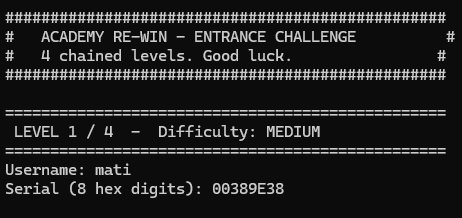
\includegraphics[width=0.7\linewidth]{initial/img/level1.png}
\caption{Level 1 screen: username and serial entered}
\label{fig:level1}
\end{figure}

\subsection{Static analysis}
% How the validation routine was located: strings, cross-references, relevant functions.
\textit{[To be completed.]}

\subsection{Dynamic analysis}
% Breakpoints used, registers/memory observed at the comparison.
\textit{[To be completed.]}

\subsection{Validation algorithm}
% Pseudocode of the rebuilt algorithm.
\textit{[To be completed.]}

\subsection{Solution (keygen)}
\textit{[To be completed.]}

\begin{lstlisting}[language=Python]
# Keygen - Level 1
# TODO: paste the keygen code
\end{lstlisting}

\subsection{Result}
The binary accepts the credential: the input is shown in Figure~\ref{fig:level1} and the \texttt{Level 1 PASSED} message at the top of Figure~\ref{fig:level2}.

\begin{lstlisting}[language={}]
Username: mati
Serial: 00389E38
[+] Level 1 PASSED
\end{lstlisting}
